% contient une description du fonctionnement de Szeliski, pour préciser qu'on possède une méthode "parfaite" dans le cas des affinités

%Le traitement par décomposition des homographies utilise une méthode de traitement des affinités. Elle est présentée dans la partie ci-dessous.

Affinities are a particular case of homographies for which there exists a efficient anti-aliasing method, and which will be used later to resample all homographies.

\subsection{Principle}
	
	This multi-pass resampling method has been introduced by Szeliski, Winder et Uyttendaele \cite{szeliski2010high}. It has been thought to minimize apparition of aliasing.

	%Le principe de cette méthode est d'abord de se ramener à des affinités qui n'agissent que selon une direction (affinités de la forme $\pmatrice{a_0 & a_1 & t\\ 0 & 1 & 0}$ ou $\pmatrice{1 & 0 & 0\\ a_1 & a_0 & t}$). Par abus de langage, on parlera de \emph{shear}, bien qu'il s'agisse de la composée d'un cisaillement, d'une dilatation unidirectionnelle et d'une translation, tous dans la même direction. Chacun des \emph{shears} est ensuite effectué en trois étapes : un sur-échantillonnage dans la direction transverse, un \emph{shear} et un sous-échantillonnage dans la direction transverse.
	
	The principle is to bring back the problem to a particular case of affine map, called shear, which only act towards one direction (their matrix form is $\pmatrice{a_0 & a_1 & t\\ 0 & 1 & 0}$ or $\pmatrice{1 & 0 & 0\\ a_1 & a_0 & t}$). Each shear is computed in three steps : an upsampling, a shear and a downsampling.
	
	%Le principe de la méthode est en fait de choisir le facteur de sur-échantillonnage suffisamment grand pour que l'opération globale se fasse sans \emph{aliasing}, i.e. sans repliement du spectre (figures \ref{szeliski_decompoNaive} et \ref{szeliski_decompoSzeliski}).
	
	The aim is to choose the upsampling factor large enough so that the global operation avoids aliasing (figures \ref{szeliski_decompoNaive} et \ref{szeliski_decompoSzeliski}).
	\label{label_des_deux_prems_fig_de_szeli}
	\begin{figure}
		\centering
		\subfigure[Spectrum of the initial image]{
\includegraphics[scale=0.5]{szeliski_naiveEntree.png}}
		\subfigure[Spectrum of the final image : aliasing]{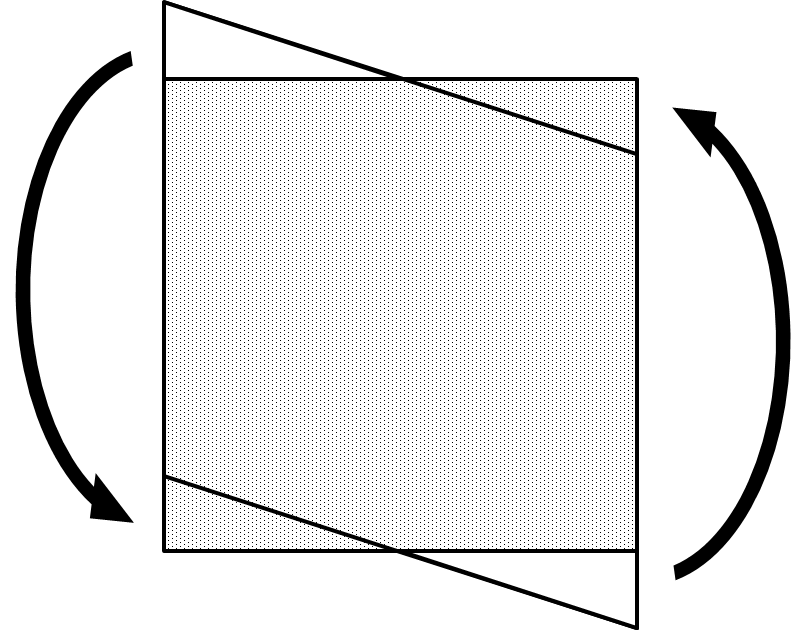
\includegraphics[scale=0.5]{szeliski_naiveSortie.png}}
		\caption{Spectrum of a naive resampling by a shear (cf. partie \ref{label_des_deux_prems_fig_de_szeli})}
		\label{szeliski_decompoNaive}
	\end{figure}
		
	\begin{figure}
		\centering
		\subfigure[Spectrum of the initial image]{
\includegraphics[scale=0.5]{szeliski_szeliskiEntree.png}}
		\subfigure[Spectrum of the image after upsampling]{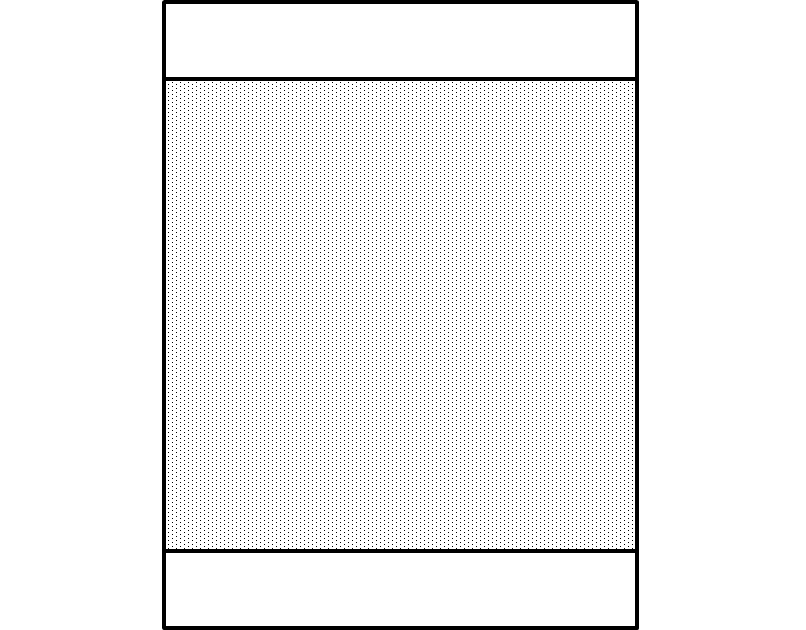
\includegraphics[scale=0.5]{szeliski_szeliskiSurechantillonnage.png}}
		\subfigure[Spectrum of the image after an upsampling and a shear]{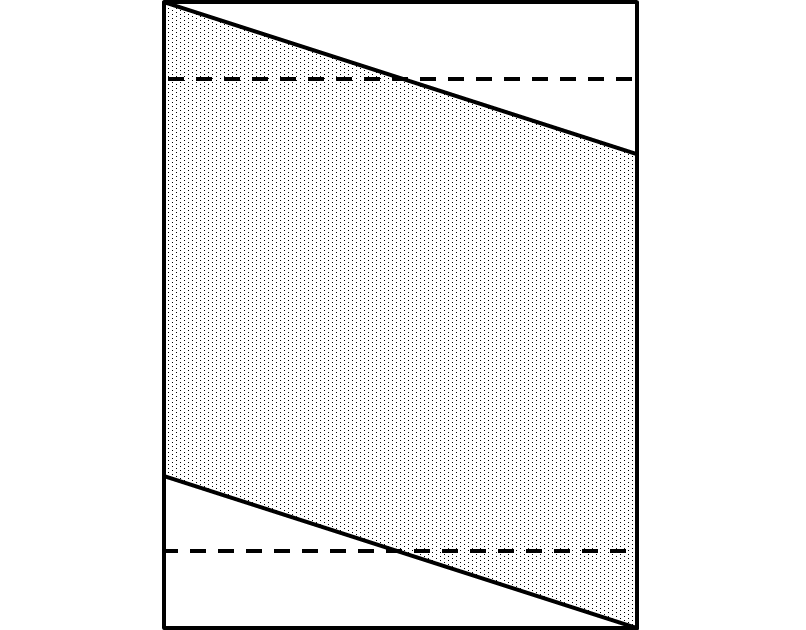
\includegraphics[scale=0.5]{szeliski_szeliskiShear.png}}
		\subfigure[Spectrum of the final image (after an upsampling, a shear and a downsampling, coupled with a low-pass filter)]{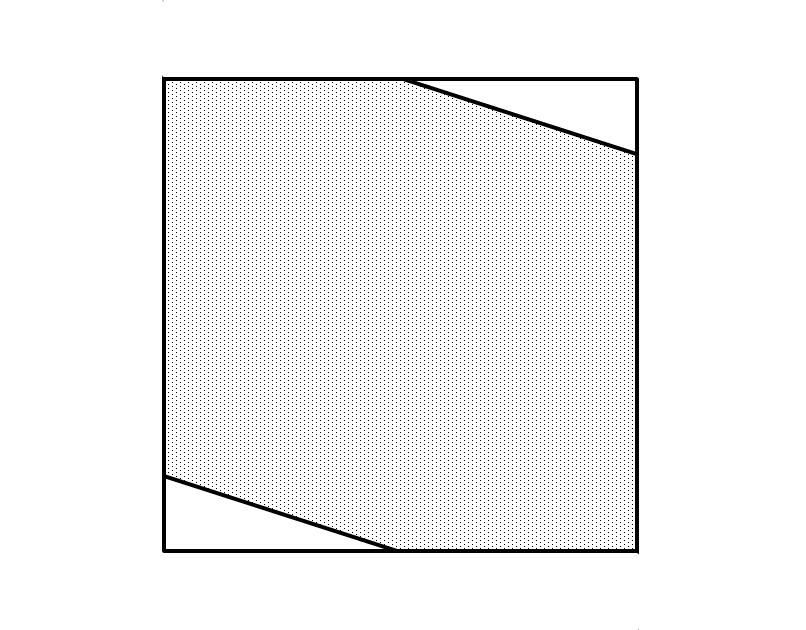
\includegraphics[scale=0.5]{szeliski_szeliskiSortie.png}}
		\caption{Spectrum of an image, resampled by a shear with the multi-pass resampling method (cf. section \ref{label_des_deux_prems_fig_de_szeli}). Experiment figure \ref{experiments_decompoSzeliski_sinc} }
		\label{szeliski_decompoSzeliski}
	\end{figure}
	
	%Ces trois opérations sont toutes des \emph{shears} (éventuellement réduits à une dilatation) et seront nommées $\mathcal R$ ; selon qu'elles modifient l'image verticalement (en laissant l'abscisse inchangée) ou horizontalement (en laissant l'ordonnée inchangée), on parlera de $\mathcal R_v$ ou de $\mathcal R_h$ . Ces opérations $\mathcal R$ sont réalisées par une convolution par un noyau d'interpolation, en l'occurrence une fonction de type \emph{raised cosine-weighted sinc}, pour pouvoir atténuer, voire supprimer, les fréquences au-delà d'un certain seuil.
	
	Those three operations are all shears (eventually reduced to a dilatation) and will be called $\mathcal R$ ; depending on what direction they modify (vertically or horizontally), 	they are called $\mathcal R_v$ or $\mathcal R_h$. Those operations $\mathcal R$ are done by convolving with a interpolation kernel, a raised cosine-weighted sinc, to extenuate or delete frequences beyond a threshold.
	
	\begin{equation}
	h : x \mapsto \sinc(\frac{x}{T})\frac{\cos(\frac{\pi\beta x}{T})}{1-\frac{4\beta^2x^2}{T^2}}
	\label{szeliski_definition_raisedCosineWeightedSinc}
	\end{equation}
	The period $T$ is equal to one (the size of a pixel).
	The parameter $\beta$, called roll-off factor, is a crucial choice. If $\beta$ is around $0.36$ (which the parameter used for most of the experiments in appendix), the support of $h$ can be reasonably approximated as contained in $[-4,4]$, and so the convolution reduces to a sum of nine terms (figure \ref{szeliski_plotRaisedCosine}), as long as the support is not modified.
	
	
%	Le paramètre $\beta$, intitulé \emph{roll-off factor}, peut varier. En prenant $\beta$ autour de $0.36$ (paramètre utilisé pour la plupart des expériences en annexe), on peut considérer que le support de $h$ est compris dans $[-4,4]$, et donc réduire la convolution à une somme d'au plus neuf termes (figure \ref{szeliski_plotRaisedCosine}), tant que le support du filtre n'est pas modifié.
	\label{label_figure_dom_reel_fourier_jt}
	\begin{figure}
		\centering
		\subfigure[Space domain]{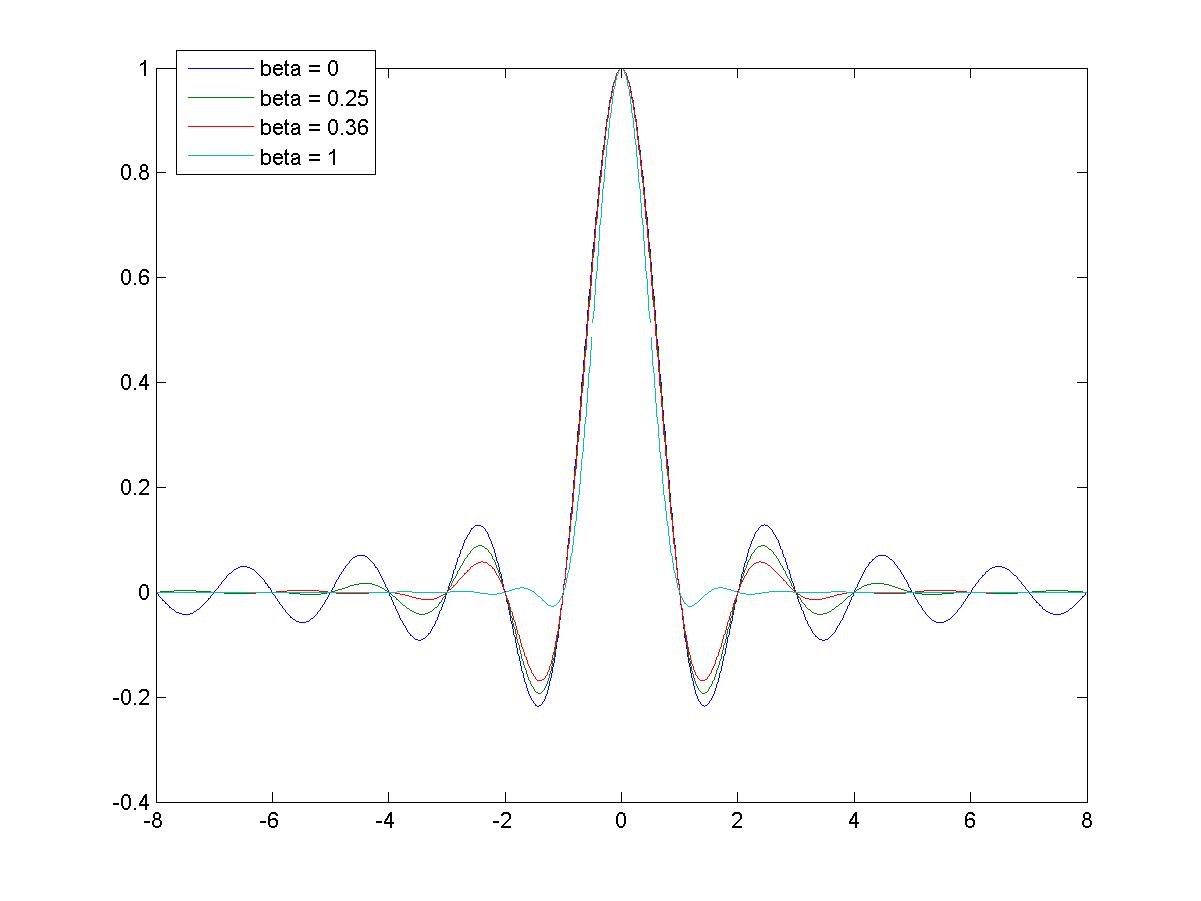
\includegraphics[scale=0.3]{raisedCosine-weightedSinc.jpg}}
		\subfigure[Frequency domain]{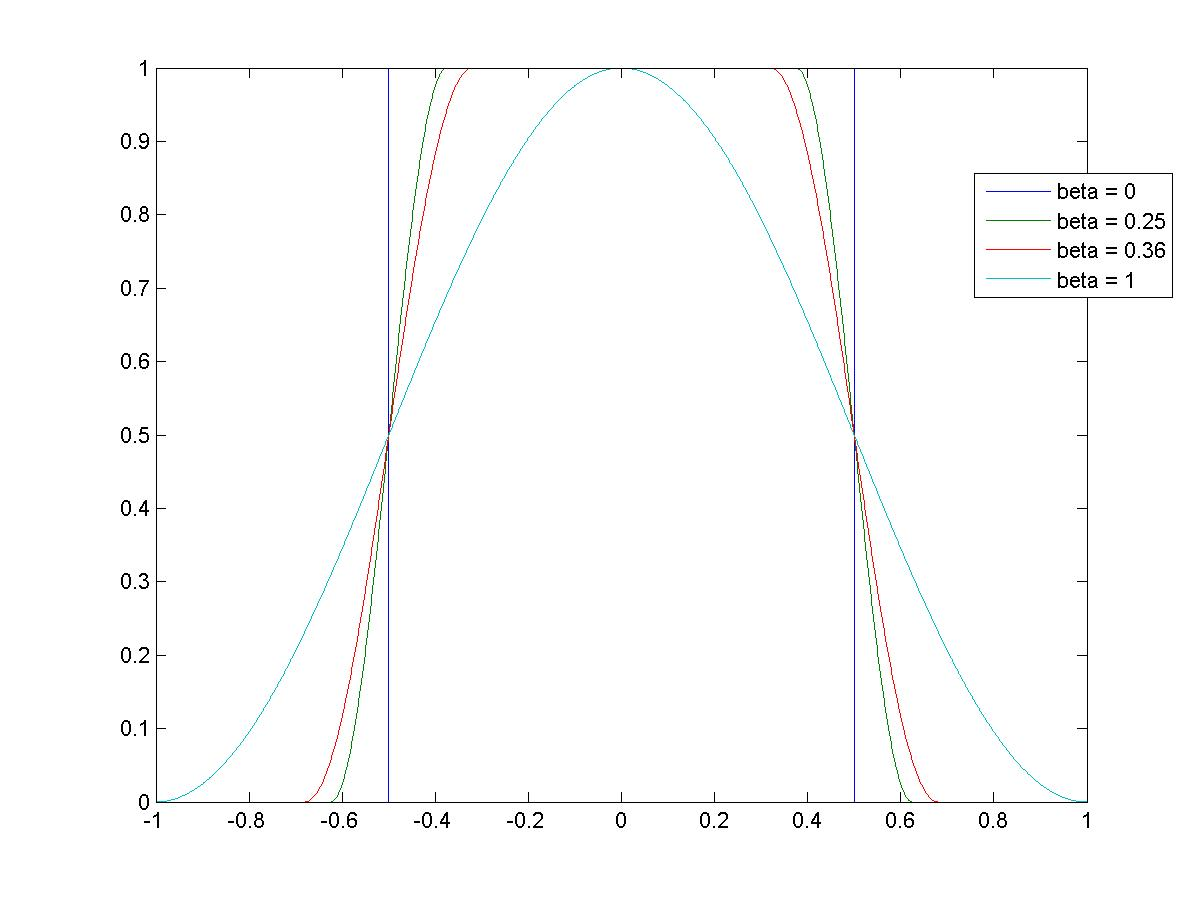
\includegraphics[scale=0.3]{raisedCosine-weightedSinc_spectrum.jpg}}
		\caption{Representations of the \emph{raised cosine-weighted sinc} filter with different parameters $\beta$ (cf. section \ref{label_figure_dom_reel_fourier_jt})}
		\label{szeliski_plotRaisedCosine}
	\end{figure}
	
	In practice, the support of the filter vary, depending on the zoom factor $s$, hence the formula to convolve with $h$ (here horizontally)
	\begin{equation}
	img_f[i][j] = \displaystyle{\sum_k}h\left(\frac{a_0i+a_1j+t-k}{s}\right)img[k][j]
	\label{formule_convolution_discrete}
	\end{equation}
	where $img_f$ is the output image and $img$ the input image.
	
	
%	En pratique, le support du filtre est adaptatif, et dépend d'un facteur de zoom $s$, d'où la formule de convolution par $h$ (ici convolution selon les abscisses) :
%	où $img_f$ est l'image finale et $img$ l'image initiale.
	
	Multiplying by $s$ the size of support of the filter function (by calling $h(\frac{x}{s})$ instead of $h(x)$, with $s\geq 1$) divides by $s$ the bandwidth of this filter. This protects against aliasing during downsamplings. The coefficient $s$ also depends on the \emph{maximal preserved frequencies} $u_{max}$ and $v_{max}$ which will be presented later.
	
%	En multipliant par $s$ la taille du support du filtre (en appelant $h(\frac{x}{s})$ au lieu de $h(x)$, avec $s\geq 1$), on divise par $s$ la largeur de la bande passante de ce filtre. Cela permet, lors d'un sur-échantillonnage, d'avoir une protection contre l'\emph{aliasing}. Le coefficient $s$ dépend aussi des \emph{fréquences conservées maximales} $u_{max}$ et $v_{max}$ qui seront définies et expliquées plus loin.
	
	The algorithms \ref{szeliski_rh} and \ref{szeliski_rv} dealing with the $\mathcal R_h$ and $\mathcal R_v$ operations are obtained by applying the formula \ref{formule_convolution_discrete} for every $i$ and $j$ in the output image. \label{szeliski_rv_rh_section}
	
%	En appliquant la formule précédente pour toutes les valeurs de $i$ et $j$ de l'image d'arrivée, on obtient les algorithmes \ref{szeliski_rh} et \ref{szeliski_rv} traitant les opérations $\mathcal R_h$ et $\mathcal R_v$. \label{szeliski_rv_rh_section}
	
	So it is possible to compute, in three steps $\mathcal R$ and without aliasing, any shear. Since an affinity can be decomposed in two shears (proposition \ref{propositionDecompositionAffinite}), any affinity can be processed without aliasing (algorithme \ref{szeliski_affine}).
	
%	On est ainsi capable d'effectuer, en trois étapes $\mathcal R$ et sans \emph{aliasing}, tous les \emph{shears}. Or une affinité se décompose toujours en deux \emph{shears} (proposition \ref{propositionDecompositionAffinite}), on peut donc toujours traiter une affinité quelconque, et ce, sans \emph{aliasing} (algorithme \ref{szeliski_affine}).

	\begin{thm}
	The multi-pass resampling method \cite{szeliski2010high} prevents aliasing while preserving as much of the spectrum as possible. %SHMUEL RELIT STP, je ne savais pas traduire
%	Le méthode multi-étapes \cite{szeliski2010high} empêche le repliement du spectre tout en conservant le maximum du spectre.
	\end{thm}
	\begin{proof}
	The effect of the different steps on the spectrum is presented figure \ref{szeliski_decompoSzeliski} and experimentally verified figure \ref{experiments_decompoSzeliski_sinc}.
	
	The downsampling is processed without aliasing by expanding the support of the filter $h$.
	\end{proof}
	
	%\begin{proof}
%	L'effet des différentes étapes sur le spectre est présenté en figure \ref{szeliski_decompoSzeliski} et vérifié en pratique figure \ref{experiments_decompoSzeliski_sinc}.
	
%	Le sous-échantillonnage est effectué sans repliement grâce à un élargissement du support du filtre $h$ (support adaptatif).
	%\end{proof}
	
	\emph{A priori} this method decomposes any affinity in six steps $\mathcal R$ (three per shears). In fact it is possible to merge some $\mathcal R$ if they act in the same direction. The decomposition can then be reduced to four steps $\mathcal R$ : a vertical up-sampling, an horizontal shear, a vertical shear and finally an horizontal downsampling.
	
%	Cette méthode semble donc décomposer une affinité en six opérations $\mathcal R$ (trois pour chacun des deux \emph{shears}) ; en pratique, il est possible de réunir certains $\mathcal R$, s'ils sont dans la même direction. La décomposition peut alors se réduire à quatre opérations $\mathcal R$ : un sur-échantillonnage vertical, un \emph{shear} horizontal, un \emph{shear} vertical puis enfin un sous-échantillonnage horizontal.
	
\subsection{Steps of the algorithm}
	\label{szeliski_affine_section}
	
	The details of the processing of the steps of the multi-pass resampling algorithm for affinity are described in this section. The corresponding algorithms can be found in appendix (algorithms \ref{szeliski_affine} and following).
	
	Let $A$ be the matrix of the inverse affinity of the one supposed to be processed. Let's denote

\[A = \pmatrice{a_{00} & a_{01} & t_0\\ a_{10} & a_{11} & t_1}\]

%	On détaille donc ici les étapes de l'algorithme de traitement d'une affinité par cette méthode multi-étape. Le pseudo-code correspondant est présent en annexe (algorithmes \ref{szeliski_rh}, \ref{szeliski_rv} et \ref{szeliski_affine}).
	
%	On suppose avoir reçu en entrée une image à modifier et la matrice $A$ correspondant à l'affinité inverse de celle à effectuer : l'antécédent du point $(i,j)$ de l'image de sortie se situe donc en $A(i,j)$ sur l'image d'entrée.
	
%	On notera
	
	\subsubsection{Eventual transposition}
		\label{szeliski_transpoOpt_section}
		
		The $\mathcal R$ can compress the image on a few pixels and then expand it (e.g. when $A$ is a rotation of angle $\frac{\pi}{2}$), this is called the bottleneck problem \cite{wolberg1990digital}.

%	Les $\mathcal R$ peuvent, si l'affinité est par exemple une rotation d'angle $\frac{\pi}{2}$, compresser l'image sur peu de pixels puis tenter de la dilater ; cet effet est un \emph{bottleneck problem} déjà connu \cite{wolberg1990digital}.
		
		To prevent this, the image and the matrix can be transposed. Let's denote
		
	%	On effectue donc éventuellement une transposition (de l'image et de la matrice) pour éviter cet effet : en notant
		\[\hat a_{00} = \frac{a_{00}}{\sqrt{a_{00}^2+a_{11}^2}}\]
		\[\hat a_{01} = \frac{a_{01}}{\sqrt{a_{00}^2+a_{11}^2}}\]
		\[\hat a_{10} = \frac{a_{10}}{\sqrt{a_{10}^2+a_{11}^2}}\]
		\[\hat a_{11} = \frac{a_{11}}{\sqrt{a_{10}^2+a_{11}^2}}\]
		%on transpose dans le cas où $|\hat a_{00}|+|\hat a_{11}|<|\hat a_{01}|+|\hat a_{10}|$.
		the transposition is done when $|\hat a_{00}|+|\hat a_{11}|<|\hat a_{01}|+|\hat a_{10}|$.
		It corresponds to the algorithm \ref{szeliski_transpoOpt}.
		%Cette transposition correspond à l'algorithme \ref{szeliski_transpoOpt}.
		
	\subsubsection{Decomposition of $A$}
		\label{szeliski_decompositionDeA_section}
		\label{szeliski_frequencesMax_section}
		
		The \emph{maximal preserved frequency}  $u_{max}$ and $v_{max}$ are the frequencies beyond which the spectrum will be erased by the application of $A$. They are defined in the frequency domain by the figure \ref{uMax_vMax}. Frenquencies beyond them can be filtered without altering the output spectrum. These definitions assume that the spectrum has been normalized on the square $[-1,1]^2$.
		
%		On introduit les fréquences conservées maximales $u_{max}$, $v_{max}$ : ce sont les fréquences, horizontales et verticales, au delà desquelles les fréquences seront effacées par l'application de $A$ ; elles sont donc définies dans le domaine de Fourier par la figure \ref{uMax_vMax}. Les fréquences au-delà de $u_{max}$ horizontalement et de $v_{max}$ verticalement peuvent donc être filtrées, cela ne changera pas le spectre de sortie. Ces définitions se font après après avoir ramené le spectre sur le carré $[-1,1]^2$.
		
		\begin{figure}
		\centering
		\subfigure[Spectrum of the input image]{
\includegraphics[scale=0.5]{uMax_vMax_spectreEntree.png}}
		\subfigure[Spectrum of the output image]{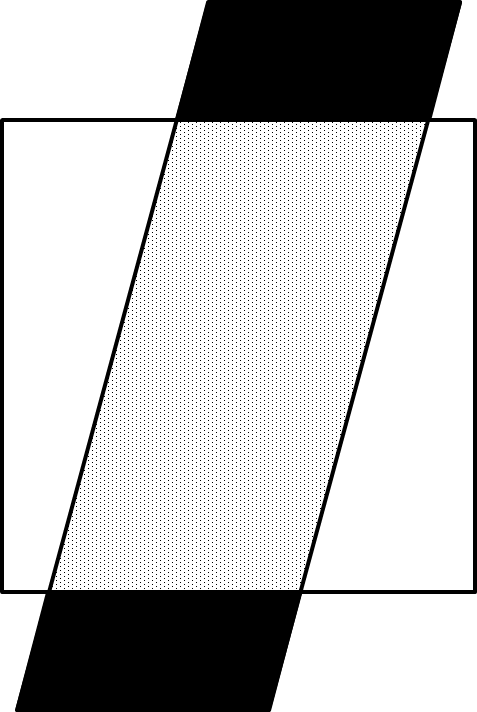
\includegraphics[scale=0.5]{uMax_vMax_spectreSortie.png}}
		\subfigure[Spectrum of the input image]{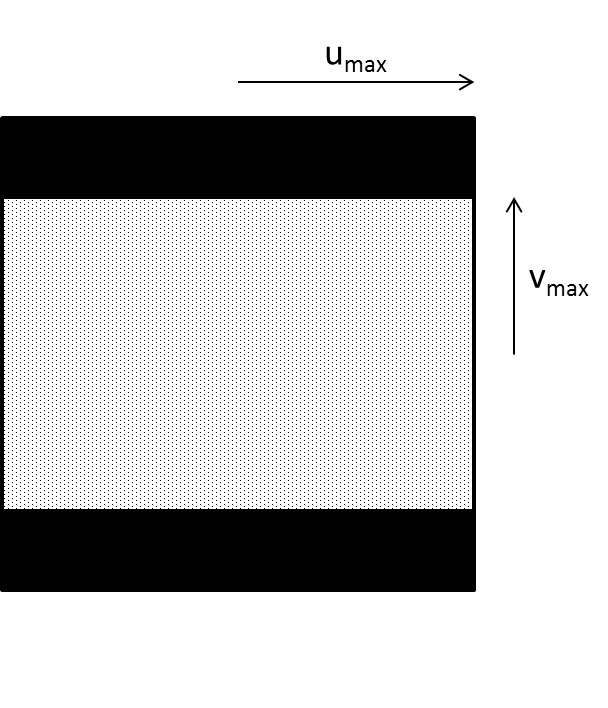
\includegraphics[scale=0.5]{uMax_vMax_spectreUtile.png}}
		\caption{Frequencies preserved by the affinity. The dark areas corresponds to frequencies erased}
		\label{uMax_vMax}
		\end{figure}
		
 
		 $u_{max}$ and $v_{max}$ can be found by finding the intersection of the input spectrum (that is to say the square $[-1,1]^2$) and the inverse image of the square by $^t\!A$ (because doing  $^t\!A$ in the frequency domain is equivalent to do $A^{-1}$ in the spatial domain ; as before $A$ is the inverse of the affinity applied to the input image). The algorithms \ref{szeliski_intersectionsVerticales} and \ref{szeliski_intersectionsHorizontales} make the intersection of a segment (which bounds are $(U_1,V_1)$ and $(U_2,V_2)$) and one of the sides of the square $[-1,1]^2$. Those two algorithms are used in the algorithm \ref{pseudo-code_umax_vmax} to compute $u_{max}$ and $v_{max}$.


		%En pratique, $u_{max}$ et $v_{max}$ s'obtiennent en intersectant le spectre d'entrée (le carré $[-1,1]^2$) et l'image réciproque du carré $[-1,1]^2$ par $^t\!A$ (qui correspond à l'opération dans Fourier ; comme précédemment $A$ désigne l'inverse de l'affinité qu'on applique à l'image). Les algorithmes \ref{szeliski_intersectionsVerticales} et \ref{szeliski_intersectionsHorizontales} réalisent l'intersection d'un segment (d'extrémités $(U_1,V_1)$ et $(U_2,V_2)$) et d'un côté du carré $[-1,1]^2$. L'algorithme \ref{pseudo-code_umax_vmax} s'appuie sur ces algorithmes pour calculer $u_{max}$ et $v_{max}$.
		
		From $A$'s coefficients and the values of $u_{max}$ and $v_{max}$, the coefficients of the vertical upsampling and the horizontal one can be deduced \cite{szeliski2010high} as follows,
		\[r_v \geq \max (1,|a_{01}|u_{max}+\min (1,|a_{11}|v_{max}))\]
		\[r_h \geq \max (1,|a_{10}/a_{11}|r_vv_{max}+\min (1,|b_0|u_{max})).\]

		%À partir des coefficients de $A$ et des valeurs de $u_{max}$ et $v_{max}$, on peut en déduire les coefficients de sur-échantillonnage verticaux et horizontaux nécessaires \cite{szeliski2010high} :
		%\[r_v \geq \max (1,|a_{01}|u_{max}+\min (1,|a_{11}|v_{max}))\]
		%\[r_h \geq \max (1,|a_{10}/a_{11}|r_vv_{max}+\min (1,|b_0|u_{max}))\]

		By geometric condiderations, one can always reduces the upsamplings to $r_h \leq 3$ and $r_v \leq 3$. Indeed, in both unidirectional mappings (those splitted into three $\mathcal R$), $r_h$ and $r_v$ can be reduced to three, thanks to the filtering which attenuates the frequencies beyond $u_{max}$ and $v_{max}$ respectively. The figure \ref{rvleq3} presents that geometric reasoning for a mapping on columns (which is a mapping on rows in the frequencie domain).

		%Pour des raisons géométriques, on peut toujours réduire les sur-échantillonnages à $r_h \leq 3$ et $r_v \leq 3$. En effet, pour chacune des deux opérations unidirectionnelles (celles qui seront décomposées en trois $\mathcal R$), le $r_h$ (respectivement $r_v$) peut être réduit à 3, grâce au filtrage qui atténue les fréquences au delà de $u_{max}$ (respectivement $v_{max}$). La figure \ref{rvleq3} présente ce raisonnement géométrique pour une opération sur les colonnes (qui se traduit par une opération sur les lignes dans le domaine de Fourier).
		
		\begin{figure}
		\centering
		\subfigure[$r_v$ not bounded]{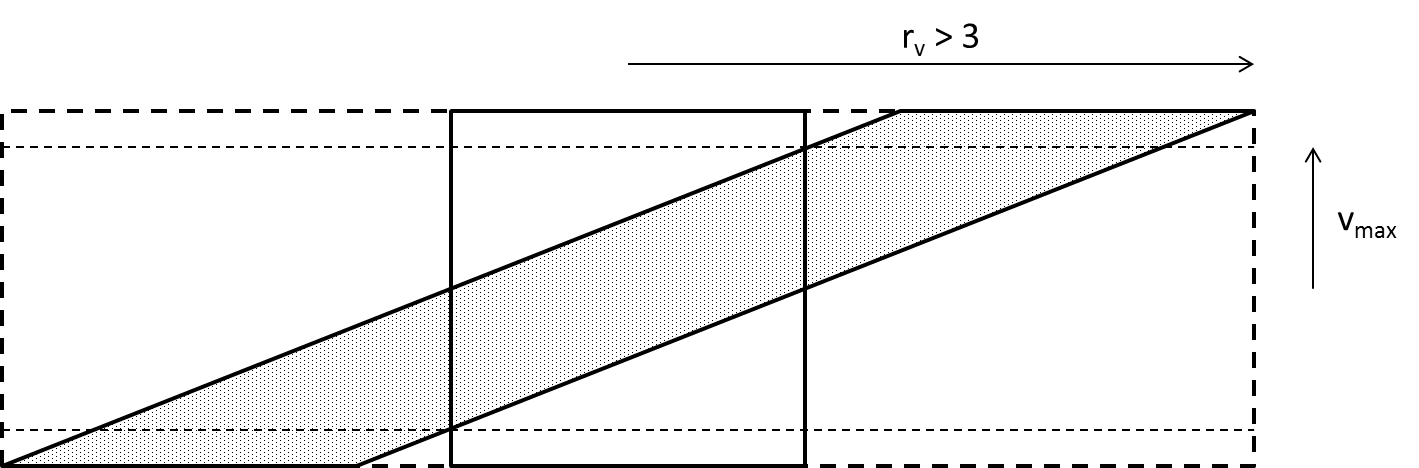
\includegraphics[width=120mm]{rvleq3_notrvleq3.png}}
		\subfigure[$r_v$ bounded by 3 ; the fact the horizontals spacings are unchanged has been used]{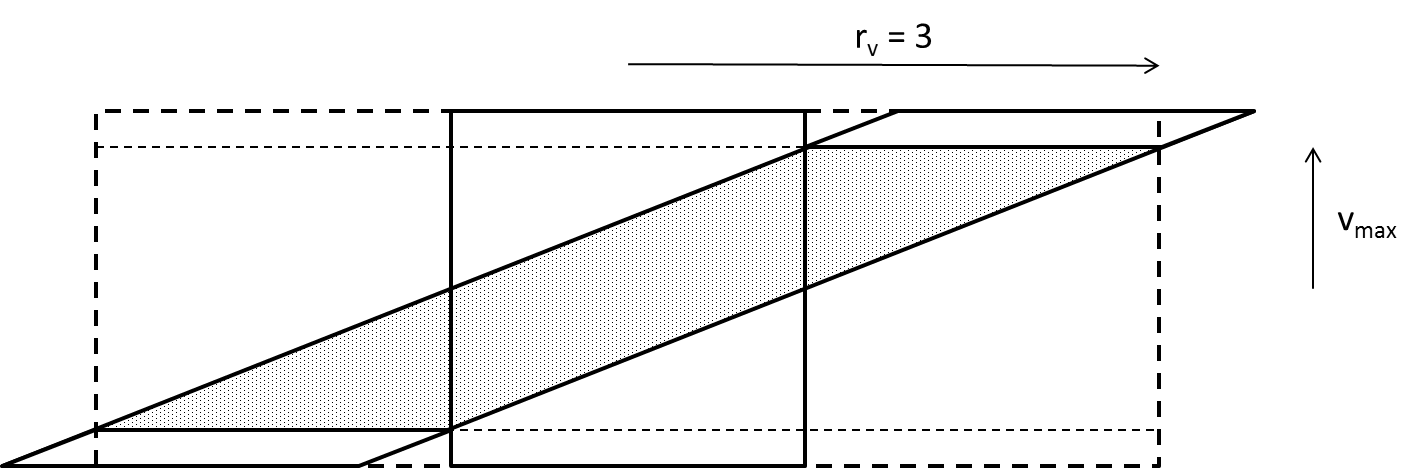
\includegraphics[width=120mm]{rvleq3_rveq3.png}}
		\caption{Reduction of $r_v$ down to $r_v \leq 3$. Beyond $v_{max}$, the frequencies are filtered. $s$ is the parameter of the filter which reduces the bandwidth. Then the $r_v$ needed to avoid aliasing can be reduced. $r_v$ is the ratio of the length of the dotted rectangle (which is the spectrum after the upsampling) and that of the square (which is the initial spectrum)}
		\label{rvleq3}
		\end{figure}


		\begin{prop}
		\label{propositionDecompositionAffinite}
		Let $A$ be an affine transform given with it's projective form, $A = \pmatrice{a_{00} & a_{01} & t_0\\ a_{10} & a_{11} & t_1\\ 0&0&1}$.
		%Soit $A$ une affinité donnée sous forme projective : $A = \pmatrice{a_{00} & a_{01} & t_0\\ a_{10} & a_{11} & t_1\\ 0&0&1}$.
		
		$A$ can be split as follows,
		%$A$ se décompose de la manière suivante :
		\[
			A = 
			\pmatrice{1 & 0 & 0\\ 0 & \frac{a_{11}}{r_v} & 0\\ 0 & 0 & 1}
			\pmatrice{\frac{b_{0}}{r_h} & \frac{a_{01}}{r_v} & t_2\\ 0 & 1 & 0\\ 0 & 0 & 1}
			\pmatrice{1 & 0 & 0\\ \frac{a_{10}r_v}{a_{11}r_h} & r_v & \frac{t_1r_v}{a_{11}}\\ 0 & 0 & 1}
			\pmatrice{r_h & 0 & 0\\ 0 & 1 & 0\\ 0 & 0 & 1}
		\]
where $b_0 = a_{00} - \frac{a_{01}a_{10}}{a_{11}};$ et : $t_2 = t_0 - \frac{a_{01}t_1}{a_{11}}$.
\end{prop}
	\subsubsection{The $\mathcal R$ mappings}
	%\subsubsection{Applications des $\mathcal R$}
		
		All that remains is to do the four $\mathcal R$ mapping.
		%Il ne reste qu'à appliquer les quatre opérations $\mathcal R$.
		
		For each ones, the first step is to keep in memory all the values of $h(\frac{k+\varphi}{s})$ with
		%Pour chacune, on commence par stocker les différentes valeurs de $h(\frac{k+\varphi}{s})$ où :
		
\begin{itemize}
		\item $\varphi \in  \frac{l}{2^b}, l \in \left\lbrace \llbracket 0,2^b-1\rrbracket \right\rbrace$ with $b$ the number of precision bit needed.
		\item $k$ is an integer such that $\frac{k}{s}$ is in the support of $h$ ($h(x)$ being nearly zero if $|x|$ is large enough, one assumes that $h$ is compactly supported).
		\end{itemize}
		Thus all the values of $h$ used for the convolution can be easily found.



%\begin{itemize}
%		\item $\varphi$ parcourt $2^b$ nombres rationnels de $[0,1]$ avec $b$ le nombre de bit de précision voulu
%		\item $k$ parcourt les entiers tels que $\frac{k}{s}$ soit dans le support de $h$ ($h(x)$ étant presque nul quand $|x|$ est assez grand, on suppose %$h$ à support compact)
%		\end{itemize}
%		On a ainsi accès rapidement à toutes les valeurs de $h$ qui peuvent être nécessaires à la convolution.
